\chapter{Le formulaire funéraire}\label{ch:formulaire}

\section{Une règle de relevé unique}

Le relevé du formulaire distingue trois situations que la notation épigraphique sépare et que les comptages confondent souvent : une expression gravée en toutes lettres ; une expression abrégée sur la pierre, dont le développement est éditorial ; une expression dont tout ou partie des lettres est restitué dans une lacune. Dans \emph{in p(ace)}, l’abréviation est gravée et seul le développement appartient à l’éditeur ; dans \emph{in [pace]}, les lettres du second mot sont absentes du support. Une quatrième situation, plus rare, est celle de la correction éditoriale : \emph{i⸢n⸣ pace} signale une lettre gravée différente de la lettre attendue (M pour N aux \nnums{121} et 150), non une lacune.

Chaque élément du formulaire est recherché par une expression régulière appliquée au texte normalisé (\emph{u/v} et \emph{i/j} unifiés), et chaque occurrence reçoit le statut de ses lettres. Une expression interrompue par une fin de ligne (\emph{pa/ce}) est reconnue comme une seule occurrence. Un texte est compté « sans restitution » lorsqu’au moins une occurrence de l’élément ne comporte aucune lettre restituée ; il est compté « avec restitution » lorsqu’au moins une occurrence, restituée ou non, est présente. Les règles exactes, les formes relevées et les notices concernées sont publiées au chapitre~\ref{ch:rep_formulaire}.

\section{La formule \emph{in pace}}

Dans l’ensemble C, \emph{in pace} est attestée dans \st{ip_tot} textes (\st{ip_pct}~\%), répartis en quatre groupes exclusifs (figure~\ref{fig:inpace}) :

\begin{itemize}
\item \st{ip_ecrit} textes la donnent en toutes lettres, sans lettre corrigée (\st{ip_ecrit_pct}~\% de l’ensemble) ;
\item \st{ip_abrege} textes la donnent abrégée (\emph{in p(ace)}), sans restitution ni correction ;
\item \st{ip_corrige} textes la donnent avec une correction éditoriale, sans restitution (\nnums{76}, 121, 150 et 359) ;
\item \st{ip_restitue} textes ne l’attestent que par une restitution.
\end{itemize}

\begin{figure}[tbp]\centering
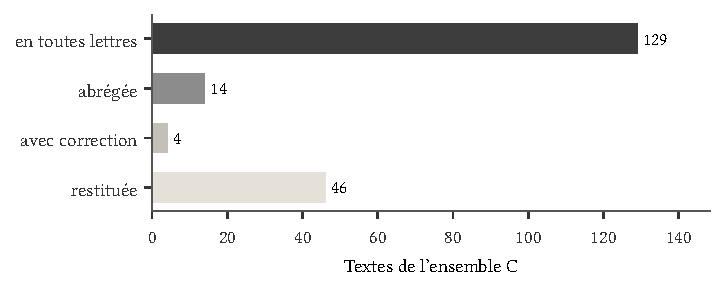
\includegraphics[width=0.7\linewidth]{figures/fig_inpace.pdf}
\caption{La formule \emph{in pace} dans l’ensemble C : quatre catégories exclusives (n = \st{ip_tot}).}\label{fig:inpace}
\end{figure}

Près d’un quart des attestations repose donc sur une restitution. Ces restitutions ne sont pas arbitraires : la formule est si fréquente que les éditeurs la restituent lorsque \emph{in} ou \emph{pace} subsiste, ou lorsque l’espace et la structure du texte la suggèrent. Mais elles reproduisent, par construction, la fréquence que l’on cherche à mesurer. L’attestation sans restitution (\st{ip_sansrest} textes, 31,6~\%) est la seule base indépendante.

Sur l’ensemble initial de 468 textes (C\textsubscript{0}), le même relevé donne \st{ipz_tot} attestations : \st{ipz_ecrit} en toutes lettres, \st{ipz_abrege} abrégées, \st{ipz_corrige} corrigées et \st{ipz_restitue} restituées. La version précédente du manuscrit comptait 132 attestations en toutes lettres et 46 restituées. L’écart tient à la notice 341, dont le texte commence par \emph{in p]ace} : la lacune initiale emporte le P, et l’attestation doit être classée parmi les restitutions. Le passage de C\textsubscript{0} à C (fusion des doublons, exclusion du \nnum{98}, jonction du \nnum{394}, inclusion du \nnum{406}) retire en outre deux attestations en toutes lettres et une restituée. Les listes complètes sont données ci-dessous.

% généré par scripts/04_generated.py
\begin{description}[style=nextline,leftmargin=1.5em,font=\normalfont\scshape]
\item[En toutes lettres, sans correction] (129 textes) 4, 9, 10, 16, 20, 22, 26, 28, 33, 34, 35, 38, 42, 45, 46, 47, 49, 55, 56, 57, 59, 61, 63, 68, 70, 72, 75, 78, 80, 94, 99, 102, 104, 115, 117, 119, 120, 125, 126, 127, 128, 130, 132, 133, 139, 140, 143, 144, 145, 151, 155, 156, 157, 166, 168, 172, 179, 183, 184, 185, 191, 196, 200, 202, 205, 207, 210, 211, 221, 223, 231, 233, 234, 237, 240, 241, 250, 260, 261, 271, 276, 284, 287, 288, 291, 295, 298, 300, 303, 304, 320, 323, 336, 346, 347, 351, 353, 361, 365, 367, 368, 369, 371, 374, 376, 381, 383, 388, 389, 396, 399, 402, 403, 404, 409, 411, 416, 419, 421, 427, 431, 444, 446, 448, 451, 453, 460, 463, 469.
\item[Abrégée, sans restitution ni correction] (14 textes) 17, 41, 54, 66, 81, 83, 124, 134, 203, 213, 279, 296, 420, 470.
\item[Avec correction éditoriale, sans restitution] (4 textes) 76, 121, 150, 359.
\item[Seulement avec restitution] (46 textes) 3, 6, 40, 53, 69, 73, 74, 77, 90, 93, 158, 162, 182, 186, 187, 190, 198, 226, 246, 258, 268, 272, 283, 302, 305, 322, 325, 337, 341, 343, 344, 350, 355, 362, 364, 370, 401, 408, 410, 428, 429, 430, 445, 450, 464, 471.
\end{description}


\section{Fréquences des éléments du formulaire}

Le tableau~\ref{tab:formulaire} donne, pour vingt et un éléments, le nombre de textes de l’ensemble C où l’élément est attesté, avec et sans restitution. L’écart entre les deux colonnes mesure la dépendance de chaque élément à l’égard des restitutions. Il est particulièrement élevé pour \emph{bene merenti} (86 contre 53), pour \emph{coniux} et ses équivalents (71 contre 45) et pour \emph{depositio} (247 contre 179) : ces mots occupent souvent des positions que les éditeurs restituent d’après la structure attendue du texte.

% généré par scripts/04_generated.py
\begin{table}[tbp]\centering\small
\caption{Éléments du formulaire dans l’ensemble C (n = 465) : textes où l’élément est attesté, restitutions comprises, et textes où il l’est au moins une fois sans restitution (abréviations et corrections admises).}\label{tab:formulaire}
\begin{tabular}{@{}l r r r r@{}}\toprule Élément & Avec rest. & \% & Sans rest. & \% \\\midrule
\lat{in pace} & 193 & 41,5 & 147 & 31,6 \\
\lat{depositio / depositus} & 247 & 53,1 & 179 & 38,5 \\
\lat{vixit (et variantes)} & 264 & 56,8 & 189 & 40,6 \\
\lat{bene merenti} & 86 & 18,5 & 53 & 11,4 \\
\lat{fecit / fecerunt} & 74 & 15,9 & 61 & 13,1 \\
\lat{hic (iacet, positus, requiescit…)} & 33 & 7,1 & 27 & 5,8 \\
\lat{requiescit / quiescit} & 37 & 8,0 & 29 & 6,2 \\
\lat{decessit / recessit / defunctus} & 36 & 7,7 & 28 & 6,0 \\
\lat{dormitio / dormit} & 6 & 1,3 & 3 & 0,6 \\
\lat{locus} & 26 & 5,6 & 19 & 4,1 \\
\lat{bisomus / trisomus / quadrisomus} & 10 & 2,2 & 6 & 1,3 \\
\lat{achat (emere, comparare)} & 7 & 1,5 & 4 & 0,9 \\
\lat{fossor} & 1 & 0,2 & 1 & 0,2 \\
\lat{coniux / compar / maritus / uxor} & 71 & 15,3 & 45 & 9,7 \\
\lat{virginius / virginia} & 5 & 1,1 & 3 & 0,6 \\
\lat{filius / filia} & 33 & 7,1 & 27 & 5,8 \\
\lat{parentes / pater / mater} & 29 & 6,2 & 24 & 5,2 \\
\lat{dulcissimus / carissimus} & 30 & 6,5 & 24 & 5,2 \\
\lat{plus minus} & 50 & 10,8 & 42 & 9,0 \\
\lat{se vivo / se viva} & 18 & 3,9 & 10 & 2,2 \\
\lat{post consulatum} & 23 & 4,9 & 15 & 3,2 \\
\bottomrule\end{tabular}\end{table}


Trois éléments forment le noyau du formulaire : la durée de vie (\emph{vixit}), la date de la déposition (\emph{depositus}, \emph{depositio}) et la formule \emph{in pace}. Les autres éléments sont minoritaires. La commémoration par un parent ou un conjoint (\emph{fecit}, \emph{bene merenti}), l’expression du repos (\emph{requiescit}, \emph{hic iacet}) et la mention du lieu (\emph{locus}, \emph{bisomus}) n’atteignent chacune qu’une fraction des textes.

\section{Variations chronologiques}

La figure~\ref{fig:formulaire} donne la part des textes de chaque période qui attestent l’élément sans restitution. Trois observations peuvent être formulées, avec des réserves différentes.

\begin{figure}[tbp]\centering
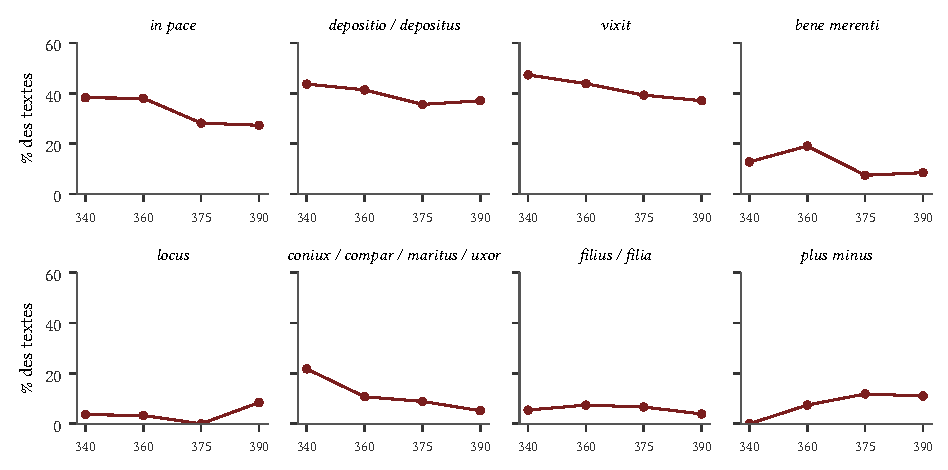
\includegraphics[width=\linewidth]{figures/fig_formulaire.pdf}
\caption{Part des textes de chaque période attestant l’élément sans restitution (ensemble C ; périodes 340–359, 360–374, 375–389, 390–403 ; effectifs \st{perC0}, \st{perC1}, \st{perC2}, \st{perC3}).}\label{fig:formulaire}
\end{figure}

\emph{Recul apparent des formules les plus fréquentes.} La part des textes portant \emph{in pace} sans restitution passe de 38~\% (21/55 ; intervalle de Wilson à 95~\% : 26,5–51,4) et 38~\% (46/121) dans les deux premières périodes à 28~\% (38/135) et 27~\% (42/154 ; 20,9–34,8) dans les deux dernières. \emph{Vixit} et \emph{depositio} reculent dans des proportions comparables. Or la part restituée des textes augmente dans le même temps : le ratio moyen de lettres restituées passe de 0,26 (340–359) à 0,29 (390–403). Avec les restitutions, la part d’\emph{in pace} est de 45~\%, 45~\%, 38~\% et 41~\% : les intervalles se recouvrent largement. Le recul apparent peut donc tenir, au moins en partie, à l’état de conservation des textes tardifs. Il ne peut être interprété comme un changement de pratique.

\emph{Recul des termes de la relation conjugale.} Les mots \emph{coniux}, \emph{compar}, \emph{maritus} et \emph{uxor} sont attestés sans restitution dans 12 textes sur 55 en 340–359 (21,8~\% ; 12,9–34,4) et dans 8 sur 154 en 390–403 (5,2~\% ; 2,7–9,9). Les intervalles ne se recouvrent pas. L’écart est plus net que pour les autres éléments, mais il repose sur de petits effectifs, et la composition topographique du corpus change entre les deux périodes (chapitre~\ref{ch:provenance}).

\emph{Apparition de nouveaux éléments dans les dernières décennies.} \emph{Plus minus} est absent des textes de 340–359 et figure dans 17 textes de 390–403 sans restitution (11,0~\%). Les mentions de l’emplacement (\emph{locus} : 13 textes en 390–403 contre 2 en 340–359), de l’achat (4 textes, tous de 390–403) et de la préparation du vivant (\emph{se vivo} : aucun texte avant 375) apparaissent ou progressent. L’expression \emph{hic iacet} et ses variantes suivent la même pente (1 texte en 340–359, 13 en 390–403). Ces observations convergent avec la chronologie admise du formulaire romain, où les mentions d’achat et d’emplacement se développent à la fin du \textsc{iv}\textsuperscript{e} siècle ; elles ne la démontrent pas à elles seules, car les effectifs restent faibles et les textes d’achat sont concentrés dans quelques secteurs.

\section{Ce que mesure le formulaire}

Le formulaire décrit des choix de rédaction et de gravure. Il ne mesure directement ni la foi des défunts, ni celle des commanditaires. La présence d’\emph{in pace} sur quatre textes sur dix est un fait de pratique épigraphique : elle associe le défunt à un vocabulaire du repos d’usage chrétien, sans préciser la nature de ce repos. Son absence ne signifie pas l’absence de conviction chrétienne : de nombreux textes très brefs ne comportent que le nom, l’âge et la date, et une partie d’entre eux porte un chrisme (chapitre~\ref{ch:supports}). Les chapitres consacrés au vocabulaire religieux (chapitres~\ref{ch:typologie} à \ref{ch:rep_religieux}) reprennent la question sur les textes qui vont au-delà du formulaire.
